\documentclass[a4paper 12pt]{article}

\usepackage[utf8]{inputenc}
\usepackage[T1]{fontenc}
\usepackage{mathptmx}
\usepackage{textcomp}
\usepackage[UKenglish]{babel}
\usepackage{amsmath, amssymb}
\usepackage{float}
\usepackage[hidelinks]{hyperref}
\hypersetup{
	colorlinks=false
}
\usepackage[style=ieee]{biblatex}
\bibliography{sources/biblio}
\renewcommand{\baselinestretch}{1.5}

\setlength{\parindent}{0pt}
\setlength{\parskip}{1em}

% figure support
\usepackage{import}
\usepackage{xifthen}
\pdfminorversion=7
\usepackage{pdfpages}
\usepackage{transparent}
\newcommand{\incfig}[1]{%
	\def\svgwidth{\columnwidth}
	\import{./figures/}{#1.pdf_tex}
}

\pdfsuppresswarningpagegroup=1

\begin{document}
\begin{titlepage}
  \begin{center}

    \textsc{\LARGE Dublin City University}\\[1cm]
    \textsc{\Large Electronic and Computer Engineering}\\[0.5cm]

    {\LARGE \bfseries EE515 Real-Time DSP: Assignment 1\\[0.4cm]}
    {\Large \bfseries The role of Digital Signal Processing in Optical
    Communications Systems\\[0.4cm]}

    \begin{figure}[H]
	
\includegraphics{images/Dcu-logo.png}
	\centering
    \end{figure}

    \vskip 2cm
    \emph{Author}\\[0.1cm]
    \noindent\makebox[\textwidth]{%
      \begin{tabular}{ll}%
        Michael Lenehan & michael.lenehan4@mail.dcu.ie \\
	Student Number: & 15410402 \\
    \end{tabular}}\\[0.1cm]

    \vfill

    % Bottom of the page
    % Probably replaced with date of deadline
    {\large{26/11/2019}}

  \end{center}
\end{titlepage}

\thispagestyle{plain}
\begingroup
\renewcommand{\cleardoublepage}{}
\renewcommand{\clearpage}{}

\LARGE{Declaration}

\endgroup

\vskip 1cm

I declare that this material, which I now submit for assessment, is entirely my
own work and has not been taken from the work of others, save and to the extent
that such work has been cited and acknowledged within the text of my work. I
understand that plagiarism, collusion, and copying are grave and serious
offences in the university and accept the penalties that would be imposed should
I engage in plagiarism, collusion or copying. I have read and understood the
Assignment Regulations set out in the module documentation. I have identified
and included the source of all facts, ideas, opinions, and viewpoints of others
in the assignment references. Direct quotations from books, journal articles,
internet sources, module text, or any other source whatsoever are acknowledged
and the source cited are identified in the assignment references. This
assignment, or any part of it, has not been previously submitted by me or any
other person for assessment on this or any other course of study.

I have read and understood the DCU Academic Integrity and Plagiarism at
\url{https://www4.dcu.ie/sites/default/files/policy/1%20-%20integrity_and_plagiarism\_ovpaa_v3.pdf}
and IEEE referencing guidelines found at
\url{https://loop.dcu.ie/mod/url/view.php?id=448779}.

\vskip 1cm
Signed: \underline{\ \ \ \ \ \ \ \ \ \ \ \ \ \ \ \ \ \ \ \ \ \ \ \ \ \ \ \ \ \ \ \ \ \ \ \ \ } \hspace{20mm}Date: \underline{08/04/2019}

\hspace*{0mm}\phantom{Signed:}Michael Lenehan

\pagebreak

\thispagestyle{plain}
\begin{center}
    \Large
    \textbf{EE-515 Real-Time DSP Assignment 1}

    \vspace{0.4cm}
    \large
    The role of Digital Signal Processing in Optical Communications Systems

    \vspace{0.4cm}
    \textbf{Michael Lenehan}

    \vspace{0.9cm}
    \textbf{Abstract}
\end{center}
\pagebreak

\tableofcontents
\clearpage
\section{Introduction}
Modern optical communications systems have been in use since the 1960's, with
the first commercial usage in 1977 in California, where telephone traffic was
transmit at a rate of 6Mbps\cite{alwayn_2004}. Since this time, systems have
been implemented to transmit data for applications such as telephony, cable
television, and internet data.
\par This literature review will present a history of the usage and
implementations of optical communications systems, and an overview of the
applications of the technology.
\par Following this, a review of the current ``state of the art'' within the
field, as it applies to digital signal processing, and the modulation algorithms
implemented, will be completed.

\section{Background}
In order to understand the ``state of the art'' within the field of optical
communications systems with relation to digital signal processing, it is
necessary to have a level of understanding of its background. This section will
introduce the basic physics concepts, a generalised overview of a typical
optical communications system, along with the advantages an optical
communication system offers.

\subsection{The Physics of Optical Communications}

Optical communications systems utilise light, typically provided by laser
diodes, or LED's, in order to transmit information along an optical fiber cable.
The optics principle of total internal reflection is utilised for the purpose of
transmission. When the incident angle of the light in the cable is greater than
the critical angle at the ``core-to-cladding interface''\cite{alwayn_2004}, the
light will reflect back into the core. This repeats thoughout the fibers core,
passing the light from source to destination.

\begin{figure}[H]
	\centering
	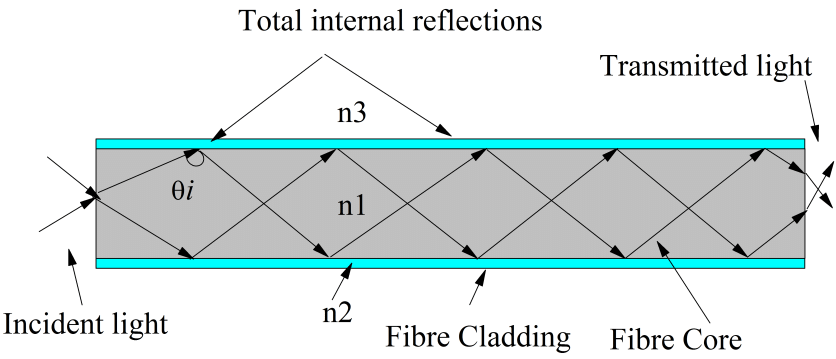
\includegraphics[width=0.8\textwidth]{images/tir}
	\caption{Total Internal Reflection within an Optical Fiber
	Cable\cite{memon_2018}}
	\label{fig:tir}
\end{figure}

\par Optical communications systems utilise light in the infrared spectrum to pass
information along a cable. The wavelength of the light in this spectrum is
in the order of thousands of micrometers ($\mu m$) in length, with frequencies
in the order of hundreds of terahertz ($\approx 10^{13}Hz$). These
high-frequency, low-wavelength carrier signals result in very high bandwidths,
and very high data transfer rates\cite{mickelson_2003}.

\par The directionality of laser light within these systems allows for greater
efficiency, as energy is not required for the filtering or correction of
divergent beams\cite{mickelson_2003}.

\subsection{Optical Communications System Overview}

Optical communications systems are typically composed of the components listed
in figure \ref{fig:overview}, that is a light source, an information source, an
encode and modulator, optics at both the transmitting and receiving side, a
transmission medium, a detector, and a receiver.

\begin{figure}[H]
	\centering
	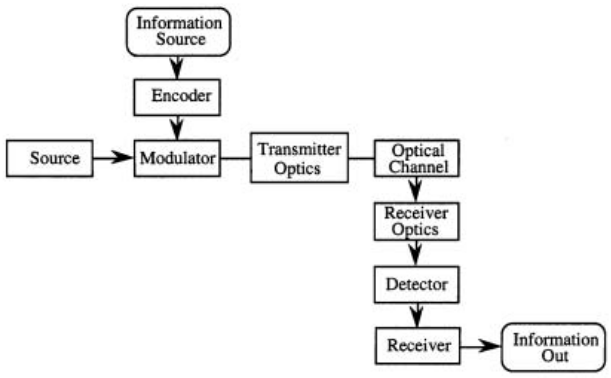
\includegraphics[width=0.8\textwidth]{images/optcommsblock}
	\caption{Generalised Block Diagram of an Optical Communications System
	\cite{mickelson_2003}}
	\label{fig:overview}
\end{figure}

\par As previously discussed, the light source used is typically an LED or a laser
diode (LD). Laser diodes offer advantages in modulation speed, power and spatial
coherence\cite{alwayn_2004}.

\par At the transmission side, the incoming source must be modulated with the data
signal. The modulation techniques used, and the most recent advances in these
techniques will be the main focus of this review paper.

\par At the receiving side, a photodiode converts the incoming light signal to
an electrical signal. This is typically followed by multiple amplication stages,
and can also include circuitry for decoding the signal, or error
detection\cite{alwayn_2004}.

\subsection{Optical Communications System Advantages}

There are many advantages to using optical communications systems over
traditional communications systems using, for example, copper wire. Optical
communications systems allow for greater resistance to interference and signal
attenuation, which can cause problems in traditional systems.

\subsubsection{Interference}

Interference can be present in traditional data transmissions through a
phenomenon known as ``Crosstalk'' which occurs when signals within different
channels of a system have an adverse, interfering effect on one
another\cite{wikipediacross_2019}. While this is an issue within the traditional
data communications systems, limiting the amount of lines which can be run in
close proximity, it poses no such issues within optical communication systems
(provided there is adequate cladding in place\cite{mickelson_2003}).

\par Optical data transmission is relatively resistant to interference, both in
terms of Electromagnetic, and Radio-Frequency interference, thus making them
more suitable than metal based, traditional transmission systems in situations
where there is high likelihood of these types of interference\cite{alwayn_2004}.

\subsubsection{Attenuation}

Attenuation in optical systems is much less of an issue than in its metal based
counterpart. This is due to attenuation being mainly caused by absorption and
scattering within the transmission medium\cite{alwayn_2004}. Within glass cable,
this attenuation is extremely low, however, with plastic core cable, it can be
higher, due to impurities within the material\cite{alwayn_2004}.

\par Attenuation within traditional systems is higher due to the ``skin effect''
which increases attenuation at higher frequencies\cite{hayt_buck_2019}. Due to
this effect, systems utilising copper wire require repeaters at approximately
2-5km intervals, compared to a distance of approximately 50km in fiber optic
cabling\cite{mickelson_2003}\cite{fiber_vs_wire}.

\section{Current State-of-the-Art}
\subsection{Modulation Techniques}

Currently there is a body of work being produced within the area of modulation
techniques for optical communications systems. One such technique, showing
promise in increasing spectral efficiency\cite{prob_2016}, while simultaneously
achieving lower optical signal to noise ratios (OSNR), and higher transmissions
distances\cite{400Gbps_2019}, is Probabilistic Shaping.

\subsubsection{Probabilistic Shaping}

Probabilistic shaping is a technique utilised for increasing spectral
efficiency within an optical communications system. Symbols are transmit via
probabilistic shaping by using non-uniform probabilities (outcomes have unequal
probabilities of occurring). Constellation points are distributed, using these
non-uniform probabilities, along the complex plane, in contrast to simpler square
quadrature amplitude modulation (QAM) constellation points, which are on a square
grid. When implemented alongside QAM this technique has been demonstrated
experimentally to give greatly increased sensitivity\cite{prob_2016}\cite{400Gbps_2019}.

\par Shaping allows for sensitivity gains of up to 0.8dB within optical
communications systems utilising 16QAM and 64QAM. In order to implement the
shaping within the system, the following probability mass function was applied:

\begin{equation}
	\label{eq:}
	P_x(x_i) = \frac{1}{\sum_{k=1}^{M} e^{-vx_k^2}}e^-vx_i^2 \quad
	\text{\cite{prob_2016}}
\end{equation}

\par In testing for mismatched SNR, the variation of SNR of 11dB was shown to not
require any modifications to the input distribution\cite{prob_2016}. This study
concluded that due to the robustness, sensitivity, and transmission distance
improvements gained from using shaping, that probabilistic shaping is ``highly
suitable for a practical application in optical communications systems''.

\par The benefits attributed to probabilistic shaping were also found in a study on
spectral efficiency in a 400Gb/s optical communications system, which found that
with probabilistic shaping alongside 64QAM, a 50\% ``reach'' improvement was
achieved over system in which probabilistic shaping was not
implemented\cite{400Gbps_2019}.

\par This study compares the efficiencies of a ``PS'' (Probabilistic Shaping)
system, versus that of a hybrid-QAM system. Hybrid QAM utilises multiple,
time-interleaved QAM's in order to improve the performance of regular QAM's. The
Maxwell-Boltzmann distribution shown below was used for the distribution of the
PS constellation points.

\begin{equation}
	\label{eq:}
	P_x(x_i) =
	\frac{\exp(-v(Re(x_i)^2+Im(x_i)^2))}{\sum_{k=1}^{M}\exp(-v(Re(x_k)^2+Im(x_k)^2))}  \quad
	\text{\cite{400Gbps_2019}}
\end{equation}

The experimental setup used, as shown in Figure \ref{fig:pstest}, shows the
utilisation of DSP techniques for the pre-transmission processing of the signal.
The input data is initially mapped to PS-64QAM symbols. These are then passed
through a pre-distortion (using look-up-tables) and pre-equalization stage. This
pre-equalization stage is composed of a 21-tap constant modulus algorithm (CMA)
Finite-Impulse-Response (FIR) filter\cite{400Gbps_2019}.

\begin{figure}[H]
	\centering
	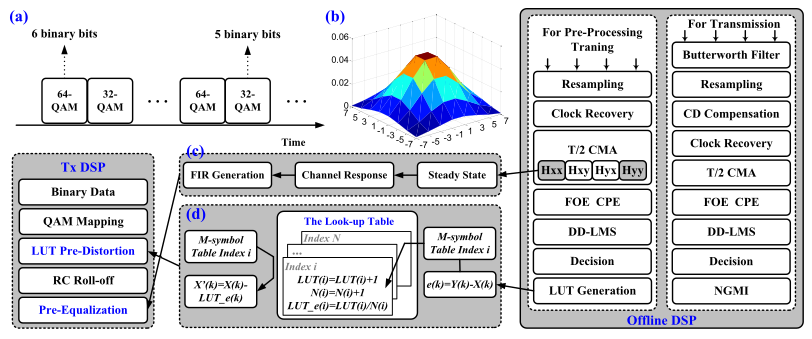
\includegraphics[width=0.8\textwidth]{images/PStest}
	\caption{Experimental Setup as in \cite{400Gbps_2019}}
	\label{fig:pstest}
\end{figure}

Due to the lower optical signal to noise ratio (OSNR) achieved using
probabilistic shaping, a transmission rate of 400Gb/s was achieved over a
transmission distance of 3,600km, a 50\% increase over the maximum transmission
distance achieved when using a hybrid-QAM system\cite{400Gbps_2019}.

\subsection{Coherent Detection and DSP}

With the increased usage of coherent detection within optical communications
systems, it has become necessary for DSP techniques to be implemented in order
to correct for transmissions errors due to the high data rates. DSP algorithms
have allowed for higher order modulation techniques than those which were
previously utilised (as discussed within the section on probabilistic shaping).
These algorithms can also allow for lower overhead within the systems, as they
can be used to mitigate the effects of, for example, chromatic dispersion,
allowing for the removal of dedicated optical dispersion compensation units from
the signal chain of the receiver\cite{100Gbaud_2019}.

\subsubsection{DSP Algorithms}

DSP algorithms allow for the mitigation or compensation of several
``impairments'' associated with coherent optical communication transmissions.
These include chromatic dispersion and polarization mode dispersion. By reducing
complexity in these systems, higher data rates can be
achieved\cite{dspcoherent}.

\par The receiver system described in Figure \ref{fig:dspcoherent} shows two fixed
equalizers, four ``butterfly-configured'' adaptive equalizers, and two phase
recovery units.

\begin{figure}[H]
	\centering
	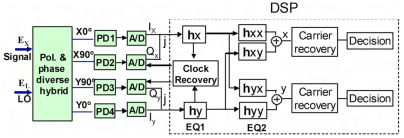
\includegraphics[width=0.8\textwidth]{images/dspcoherent}
	\caption{Generalised Digital Coherent Receiver\cite{dspcoherent}}
	\label{fig:dspcoherent}
\end{figure}

\par In order to compensate for chromatic dispersion, Fast Fourier Transform based
frequency-domain equalization can be used. Using this technique, the symbol rate
increases on a log scale, allowing for much lower complexity when compared with
a standard time-domain or frequency domain FIR filter. As such, within this
study, FFT-FDE based fixed equalizers are utilised.

\par Polarization-mode dispersion compensation is achieved using the four
adaptive equalizers. For this purpose, a T/2 spaced time-domain FIR filter
filter is used. This offers the best possible performance, however, if
complexity is a concern, a viable alternative is to use a 2T/3 FIR filter.
Using a constant modulus algorithm (CMA), the filter coefficients can be
chosen\cite{dspcoherent}.

\par The Viterbi-Viterbi (or Mth-power) method is used for the phase recovery
units. The incoming signal is raised to the $M^{th}$ power in order to remove
data modulation, and to attain the frequency offset between the transmit signal
and the local oscillator. Removing the frequency offset gives the frequency
recovered signal, to which the process is repeated in order to estimate the
phase noise, given by taking an average over multiple adjacent
symbols\cite{dspcoherent}.

\par Similar experiments have shown that the digital filtering described in
\cite{dspcoherent}, utilised in a coherent detection receiver system can achieve
high data transmission rates\cite{Savory_08}.

\subsection{Machine Learning Techniques}

Recent studies have demonstrated the benefits of machine learning techniques in
coherent optical receiver systems\cite{kMeans_2019}\cite{nn_2020}. These
techniques have been shown to give possible gain increases of approximately
2dB\cite{kMeans_2019}, or can be used for signal recovery\cite{nn_2020}.

\subsection{ML for 16-QAM Demodulation}

Machine learning techniques show promise as a replacement for the aforementioned
DSP techniques for the purpose of low complexity, high performance coherent
optical receiver systems.

\par A K-Nearest Neighbours (KNN) classification can be used for the purposes of
removing noise from a signal. Using components of each symbol of the 16-QAM
output as features, and the groups of symbols as the classes, a model can be
trained .

\par Fuzzy c-Means clustering, a version of the k-Means algorithm, calculates
the probability that an incoming signal belongs to a cluster. This, when
combined with the KNN algorithm, has been shown through simulation to give
better performance than any of the previously discussed, more traditional DSP
techniques\cite{kMeans_2019}.

\subsection{Neural Networks}

Neural networks have recently proposed as an alternative to traditional DSP
systems for low resolution analog to digital converters. This is due to the high
power consumption of high performance DSP systems within optical communication
receivers. A recent study has shown that a one-bit vertical resolution ADC, when
combined with a neural network, can recover a complex modulated
signal\cite{nn_2020}.

\par The purpose of this approach is to implement a binarized coherent optical
receiver to better utilise lower power ADC's. The binarized neural network can
allow for bitwise operations to be performed, rather than arithmetic operations,
which reduces overall memory usage\cite{nn_2020}.

\par The proposed solution in this study successfully (in simulation)
reconstructed a complex modulated signal in both a 50Gb/s SP-QPSK and 100Gb/s
PDM-QPSK system. The neural network allows for the use of lower cost ADCs, while
the reduction in memory usage and calculation complexity allows for an increase
in performance\cite{nn_2020}.

\section{Conclusions}
It is clear that there has been much work done on modulation techniques, signal
recovery, and coherent detection within the last number of years. These
techniques have allowed for benefits such as offsetting noise introduced in
transmission, reducing system complexity, increasing transmission distances, and
increase in performance.

\par While newer machine learning techniques are promising increased
performance, on lower cost, lower power ADC's, there is still work being done on
increasing performance to the greatest extent possible using more traditional
DSP techniques, as with probabilistic shaping.

\par The aim of all of the techniques mentioned is to increase data rates and
throughput within optical communications systems in an effort to increase their
usage and ubiquity in worldwide communication systems.

\clearpage
\printbibliography
\end{document}
